% 页面设置
\documentclass[12pt, a4paper]{article} % 字号:12,纸张:A4
\usepackage[top=2.54cm, bottom=2.54cm, left=3.18cm,right=3.18cm]{geometry} % 页边距设置
% 字体设置
\usepackage[UTF8]{ctex}
\usepackage{fontspec} % 设置字体
%\setCJKmainfont{SimSun}[AutoFakeBold=true, BoldFont={SimHei}, ItalicFont={KaiTi}] % 正文字体
%\setCJKsansfont[AutoFakeBold=3]{KaiTi} % 无衬线字体
%\setCJKmonofont[AutoFakeBold=3]{SimHei} % 等宽字体
\setmainfont{Times New Roman} % 设置主字体为新罗马体
% 文本设置
\usepackage{enumerate} % 支持小标题编号
\linespread{1.5} % 行间距1.5倍
\usepackage{indentfirst}%首段缩进
\setlength{\parindent}{2em} % 首行缩进两字符
\usepackage[hidelinks]{hyperref} % 目录添加超链接
\usepackage{zhnumber} % 章节标题中文显示
\usepackage[cmyk]{xcolor} % 文字彩色显示
% 数学支持
\usepackage{amsmath} % 数学公式支持
\usepackage{amssymb} % 数学符号支持
\usepackage{bm} % 公式加粗
\usepackage{mathrsfs} % 花体字母
\usepackage{yhmath} % 更多的数学符号
% 图片设置
\usepackage{caption} % 插入图片标题
\usepackage{float} % 控制图片位置
\usepackage{subfigure} % 图片并排
\usepackage{booktabs} % 插入表格
% 表格设置
\usepackage{multirow} % 表格自动换行
\usepackage{bigstrut} % 表格间距
\usepackage{rotating} % 表格旋转
\usepackage{tabularx} % 表格宽度
\usepackage{colortbl} % 表格颜色
\usepackage{graphicx} % 表格自动宽度

\title{第五章 \ \ \ 神经网络} % 文章标题
\author{Castor Ye} % 文章作者
\date{} % 文章时间

\begin{document} % 文档从这里开始。
\maketitle % 按照预定的模板把上面那些信息排好。
\newtheorem{definition}{定义}[section]
\newtheorem{theorem}{定理}[section]
\newtheorem{example}{例}[section]
\newtheorem{solution}{题解}
\newtheorem{algorithm}{算法}
\newtheorem{axiom}{公理}
\newtheorem{property}{性质}
\newtheorem{proposition}{命题}
\newtheorem{lemma}{引理}
\newtheorem{corollary}{推论}[section]
\newtheorem{remark}{注解}
\newtheorem{condition}{条件}
\newtheorem{conclusion}{结论}
\newtheorem{assumption}{假设}
\renewcommand{\figurename}{图} % 将图片序号改为图
\renewcommand{\tablename}{表} % 将表格序号改为表
%%%%%%%%%%%%%%%%%%%%%%%%%%%%%%%%%%%%%%%%%%%%%%%%%%%%%%%%%%%%%%%%%%%%%%%
% 文章内容从此开始
\section{神经元模型}

神经网络(neural networks)中最基本的成分是神经元(neuron)模型,即上述定义中的“简单单元”。在生物神经网络中,每个神经元与其他神经元相连,当它“兴奋”时,就会向相连的神经元发送化学物质,从而改变这些神经元内的电位;如果某神经元的电位超过了一个“阈值”(threshold),那么它就会被激活,即“兴奋”起来,向其他神经元发送化学物质。

\begin{figure}[H]
    \centering
    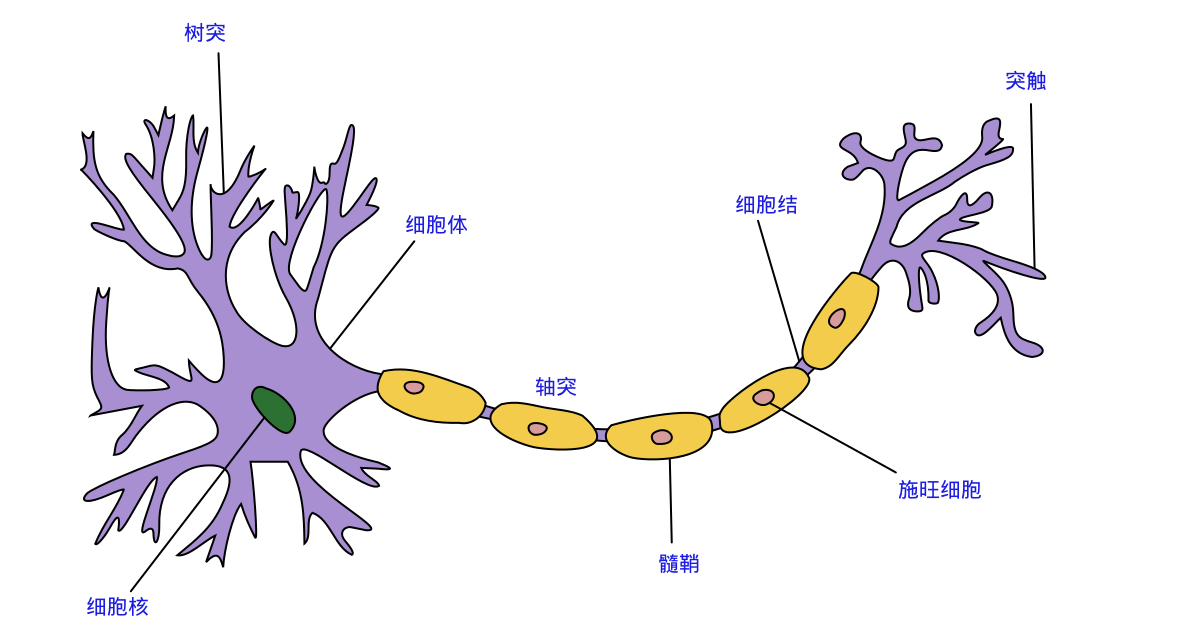
\includegraphics[width=0.8\textwidth]{../img/5-1-生物神经元.png}
    \caption{生物神经元}
    \label{fig:生物神经元}
\end{figure}

一直沿用至今的“M-P神经元模型”正是对这一结构进行了抽象,也称“阈值逻辑单元“(threshold logic unit),其中树突对应于输入部分,每个神经元收到 $n$ 个其他神经元传递过来的输入信号,这些信号通过带权重的连接传递给细胞体,这些权重又称为连接权(connection weight)。细胞体分为两部分,前一部分计算总输入值(即输入信号的加权和,或者说累积电平),后一部分先计算总输入值与该神经元阈值的差值,然后通过激活函数(activation function)的处理,产生输出从轴突传送给其它神经元。M-P 神经元模型如下图所示:

\begin{figure}[H]
    \centering
    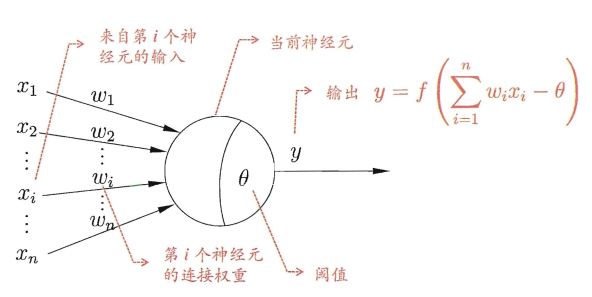
\includegraphics[width=0.8\textwidth]{../img/5-2-M-P神经元模型.png}
    \caption{M-P神经元模型}
    \label{fig:M-P神经元模型}
\end{figure}

和线性模型一样,理想中的激活函数是阶跃函数,它将输入值映射为输出值“$0$”或“$1$”。显然,“$1$”对应于神经元兴奋,“$0$”对应于神经元抑制。然而,阶跃函数具有不连续、不平滑等不太好的性质,因此实际常用 Sigmoid 函数作为激活函数。Sigmoid函数将可能在较大范围内变化的输入值挤压到 $(0, 1)$ 输出值范围内,因此也称为“挤压函数”(squashing function)。

把许多个这样的神经元按一定的层次结构连接起来,就得到了神经网络。



\section{感知机与多层网络}

感知机(Perceptron)由两层神经元组成,输入层接收外界输入信号后传递给输出层,输出层是 M-P 神经元。感知机能容易地实现逻辑与、或、非运算,注意到 $\displaystyle y = f( \sum_i w_i x_i - \theta)$,假定 $f$ 是阶跃函数,则有:

\begin{enumerate}[\hspace*{2em} i.]
    \item “与”($x_1 \wedge x_2$):令 $w1 = w2 = 1, \theta = 2$,则 $y = f(1 \cdot x_1 + 1 \cdot x_2 - 2)$,仅在 $x_1 = x_2 = 1$ 时,$y = 1$。
    \item “或”($x_1 \vee x_2$):令 $w_1 = w_2 = 1, \theta = 0.5$,则 $y = f(1 \cdot x_1 + 1 \cdot x_2 - 0.5)$,当 $x_1 - 1$ 或 $x_2 = 1$ 时,$y = 1$。
    \item “非”($\neg x_1$):令 $w_1 = -0.6, w_2 = 0, \theta = - 0.5$,则 $y = f(-0.6 \cdot x_1 + 0 \cdot x_2 + 0.5)$,当 $x_1 = 1$ 时,$y = 0$;当 $x_1 = 0$ 时,$y = 1$。
\end{enumerate}

\begin{figure}[H]
    \centering
    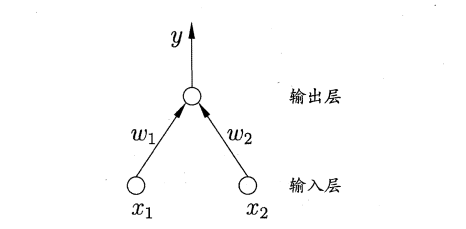
\includegraphics[width=0.5\textwidth]{../img/5-4-两个输入神经元的感知机网络结构示意图.png}
    \caption{两个输入神经元的感知机网络结构示意图}
    \label{fig:两个输入神经元的感知机网络结构示意图}
\end{figure}

更一般地,给定训练数据集,权重 $w_i(i = 1, 2, \cdots, n)$ 以及阈值 $\theta$ 可通过学习得到。阈值 $\theta$ 可看作一个固定输入为 $-1$ 的“哑结点”(dummy node)所对应的连接权重 $w_{n + 1}$,这样,权重和阈值的学习就可统一为权重的学习。感知机学习规则非常简单,对训练样例 $(x, y)$,若当前感知机的输出为 $\hat{y}$,则感知机权重将这样调整:

\begin{equation*}
    w_1 \leftarrow w_i + \Delta w_i, \ \ \ \ \Delta w_i = \eta (y - \hat{y}) x_i
\end{equation*}

其中 $\eta \in (0, 1)$ 称为学习率(learning rate)。可以看出,如果感知机对训练样例 $(x, y)$ 预测正确而,即 $\hat{y} = y$,则感知机不发生变化,否则将根据错误的程度进行权重调整。

由于感知机模型只有一层功能神经元,因此其功能十分有限,只能处理线性可分的问题,对于这类问题,感知机的学习过程一定会收敛(converge),因此总是可以求出适当的权值。但是对于像书上提到的异或问题,只通过一层功能神经元往往不能解决,因此要解决非线性可分问题,需要考虑使用多层功能神经元,即神经网络。

\begin{figure}[H]
    \centering
    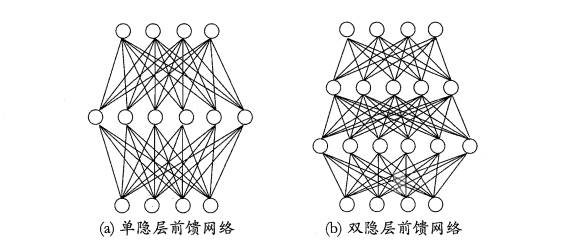
\includegraphics[width=0.8\textwidth]{../img/5-5-多层前馈神经网络结构示意图.png}
    \caption{多层前馈神经网络结构示意图}
    \label{fig:多层前馈神经网络结构示意图}
\end{figure}

在神经网络中,输入层与输出层之间的层称为隐含层或隐层(hidden layer),隐层和输出层的神经元都是具有激活函数的功能神经元。只需包含一个隐层便可以称为多层神经网络,常用的神经网络称为“多层前馈神经网络”(multi-layer feedforward neural network),该结构满足以下几个特点:

\begin{enumerate}[\hspace*{2em} i.]
    \item 每层神经元与下一层神经元之间完全互连。
    \item 神经元之间不存在同层连接。
    \item 神经元之间不存在跨层连接。
\end{enumerate}

根据上面的特点可以得知:这里的“前馈”指的是网络拓扑结构中不存在环或回路,而不是指该网络只能向前传播而不能向后传播(下节中的BP神经网络正是基于前馈神经网络而增加了反馈调节机制)。神经网络的学习过程就是根据训练数据来调整神经元之间的“连接权”以及每个神经元的阈值,换句话说:神经网络所学习到的东西都蕴含在网络的连接权与阈值中。

\section{误差逆传播算法(BP 神经网络)}

由上面可以得知:神经网络的学习主要蕴含在权重和阈值中,多层网络的学习能力比单层感知机強得多,简单感知机学习规则显然已经不够用了。误差逆传播(error BackPropagation, BP)算法正是为学习多层前馈神经网络设计,其是迄今为止最为成功的神经网络学习算法。

给定训练集 $D = \{(x_1, y_1), (x_2, y_2), \cdots, (x_m, y_m)\}, x_i \in \mathbb{R}^d, y_i \in \mathbb{R}^l$,即输入示例由 $d$ 个属性描述,输出 $l$ 维实值向量。

为便于讨论,下图给出了一个拥有 $d$ 个输入神经元、$l$ 个输出神经元、$q$ 个隐层神经元的多层前馈神经网络结构,其中输出层第 $j$ 个神经元的阈值用 $\theta_j$ 表示,隐层第 $h$ 个神经元的阈值用 $\gamma_h$ 表示。输入层第 $i$ 个神经元与隐层第 $h$ 个神经元之间的连接权为 $v_{ih}$,隐层第 $h$ 个神经元与输出层第 $j$ 个神经元之间的连接权为 $w_{hj}$。

记隐层第 $h$ 个神经元接收到的输入为 $\displaystyle \alpha_h = \sum_{i = 1}^{d} v_{ih} x_i$,输出层第 $j$ 个神经元接收到的输入为 $\displaystyle \beta_{j} = \sum_{h = 1}^{q} w_{hj}b_h$,其中 $b_h$ 为隐层第 $h$ 个神经元的输出。

\begin{figure}[H]
    \centering
    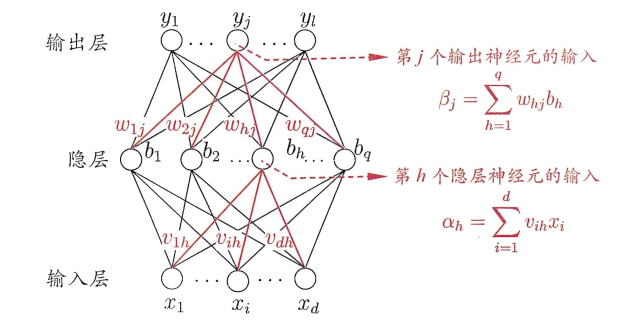
\includegraphics[width=0.8\textwidth]{../img/5-6-BP网络及算法中的变量符号.png}
    \caption{BP网络及算法中的变量符号}
    \label{fig:BP网络及算法中的变量符号}
\end{figure}

对训练例 $(x_k, y_k)$,假定神经网络的输出为 $\hat{y}_k = (\hat{y}_1^k, \hat{y}_2^k, \cdots, \hat{y}_l^k)$,即:
\begin{equation*}
    \hat{y}_j^k = f(\beta_j - \theta_j)
\end{equation*}
则网络在 $(x_k, y_k)$ 上的均方差为:
\begin{equation*}
    E_k = \frac{1}{2} \sum_{j = 1}^{l} (\hat{y}_j^k - y_j^k)^2
\end{equation*}

图 \ref{fig:BP网络及算法中的变量符号} 的网络中有 $(d + l + 1) q + l$ 个参数需确定:
\begin{enumerate}[\hspace*{2em} i.]
    \item 输入层到隐层的 $d \cdot q$ 个权值。
    \item 隐层到输出层的 $q \cdot l$ 个权值。
    \item $q$ 个隐层神经元的阈值。
    \item $l$ 个输出层神经元的阈值。
\end{enumerate}

$BP$ 是一个迭代学习算法,在迭代的每一轮中采用广义的感知机学习规则对参数进行更新估计,任意参数 $v$ 的更新估计式为:
\begin{equation*}
    v \leftarrow v + \Delta v
\end{equation*}
下面以图 \ref{fig:BP网络及算法中的变量符号} 中隐层到输出层的连接权 $w_{hj}$ 为例来进行推导。

$BP$ 算法基于梯度下降(gradient descent)策略,以目标的负梯度方向对参数进行调整,给定学习率 $\eta$,有:
\begin{equation*}
    \Delta w_{hj} = - \eta \frac{\partial E_k}{\partial w_{hj}}
\end{equation*}





\end{document}